\documentclass[11pt]{article}

% Margins
\usepackage[a4paper,
    left=2cm,
    right=2cm,
    top=2.5cm,
    bottom=2.5cm]{geometry}

\usepackage{amsmath, amssymb}
\usepackage{mathtools}
\usepackage{tcolorbox}
\usepackage{overpic}
\usepackage{float}
\usepackage{makecell}
\usepackage{etoolbox}
\usepackage{wasysym}
\robustify\diameter
\usepackage{siunitx}
\sisetup{range-phrase=\,--\,, input-comparators = \diameter}
\usepackage{hyperref}
\usepackage{booktabs}
\usepackage[dvipsnames]{xcolor}
\usepackage[
    backend=biber, style=numeric,
    sorting=none, url=false, isbn=false]{biblatex}
\addbibresource{refs.bib}
\usepackage{authblk}

\newcommand{\R}{\mathbb{R}}
\newcommand{\Z}{\mathbb{Z}}
\newcommand{\Q}{\mathbb{Q}}
\newcommand{\C}{\mathbb{C}}
\newcommand{\ii}{\mathrm{i}}
\newcommand{\mean}[1]{\overline{#1}}
\renewcommand{\bold}[1]{\mathbf{#1}}

\mathtoolsset{showonlyrefs}

\DeclarePairedDelimiter{\abs}{\lvert}{\rvert}
\DeclarePairedDelimiter{\norm}{\lVert}{\rVert}
\DeclarePairedDelimiter{\japan}{\langle}{\rangle}

\DeclareMathOperator{\BigO}{\mathcal{O}}
\DeclareMathOperator{\Exp}{\mathrm{Exp}}
\DeclareMathOperator{\E}{\boldsymbol{E}}

%--------- side numbering ------- 
\iffalse
\usepackage{tikz,everypage}
\AtBeginDocument{%
  \AddEverypageHook{%
    \begin{tikzpicture}[remember picture,overlay]
      \path (current page.north west) --  (current page.south west) \foreach \i in {1,...,\fakelinenos} { node [pos={(\i-.5)/\fakelinenos},xshift=\fakelinenoshift, line number style] {\i} }  ;
    \end{tikzpicture}%
  }%
}
\tikzset{%
  line numbers/.store in=\fakelinenos,
  line numbers=65,
  line number shift/.store in=\fakelinenoshift,
  line number shift=30mm,
  line number style/.style={text=gray},
}
\fi
%--------- side numbering ------- 

\title{DANA Article}

\author[2]{Reinaldo Espina-Navarro}
\author[1]{Mª Nieves Martínez-Alzamora}
\author[1]{José Manuel Soler-Torro}
\author[1]{Virtudes Mellado-García}

\affil[1]{Basque Center for Applied Mathematics (BCAM), Bilbao, Basque Country -- Spain}
\affil[2]{Department of Applied Statistics, Operational Research and Quality, Universitat Politècnica de València, Valencia -- Spain 
}

\setcounter{Maxaffil}{0}
\renewcommand\Affilfont{\itshape\small}

\date{\today}

\begin{document}
\maketitle

\begin{abstract}


\end{abstract}


% !TeX root = main.tex

\section{Introduction}
The floods that affected the Valencia region in October 2024 have been described as one of the most severe natural disasters in recent Spanish
history, resulting in 228 fatalities and affecting thousands of people. In such contexts of uncertainty and disruption, news media play a crucial
role in society, as they are responsible for disseminating information and shaping how events are publicly interpreted\cite{cottle,DisastersandtheMedia}.
For this reason, media coverage contributes to the construction of meaning around disasters, influencing not only how they are understood but 
also how they are socially and politically responded to.

Disasters are not only objective events defined by their material consequences but also are a socially constructed phenomena influenced
by the media representations. The way in which different media outlets select, frame, and narrate these events impacts in defining their
salience, perceived severity, and broader social implications. Rather than acting as neutral transmitters of information, media operate as 
'amplificators of risk', intensifying  




\subsection{Literature Review}


\subsection{A framework for Rhetoric Alarmism}


% !TeX root = main.tex
\section{Materials and Methods} \label{sec:materials}

\subsection{Study Design}

%\input{preprocessing}
%\input{model}
%\input{comparison}

\section{Conclusions}

We conclude that....


\subsection*{External data}

The experimetal dataset is available at....


\subsection*{Funding}


\subsection*{Acknowledgements}

The authors wish to thank ...

\printbibliography
\end{document}